\documentclass[10pt,a4paper]{article}
\usepackage[margin=2.2cm]{geometry}
\usepackage[T1]{fontenc}
\usepackage{lmodern}
\usepackage{parskip}
\usepackage{booktabs}
\usepackage{tabularx}
\usepackage{array}
\usepackage{float}
\usepackage{graphicx}
\usepackage{enumitem}
\usepackage{xcolor}
\usepackage[colorlinks=true,urlcolor=blue!60!black,linkcolor=black]{hyperref}

\graphicspath{{../payload_bench_20261124_020247/figures/}}
\newcolumntype{R}{>{\raggedleft\arraybackslash}X}

\title{Drone Authentication Study --- Step 2 Progress Report\\[3pt]
\large What happens when the signed message gets bigger, and how big can it be?}
\author{}
\date{24 November 2026}

\begin{document}
\maketitle

\section*{Summary}

When a drone proves who it is, it sends a message (its ID, a random number from the ground
station, the time, sensor readings) with a \emph{signature} attached. In Step 1 the message was
always 64 bytes. In Step 2 we made the message bigger and asked four questions. The answers:

\begin{enumerate}[nosep]
  \item \textbf{Does a bigger message take longer to sign?} Only a little. Going from 64 bytes
        to 64 KB adds about 9\,ms to Ed25519 and 6\,ms to ECDSA and RSA. ML-DSA pays more per
        extra KB (0.69\,ms), because its hashing runs in software on the ESP32.
  \item \textbf{What is the biggest message the ESP32 can sign?} 110,536 bytes, the same for all
        six algorithms. The limit is the ESP32's memory, not the algorithm.
  \item \textbf{How big a message can be signed within a time limit?} Within 100\,ms, only
        Ed25519 can always do it. ML-DSA-44 usually can, but not every time.
  \item \textbf{How much data fits next to the signature in one drone packet?} Ed25519 leaves
        191 bytes in one MAVLink packet (255 bytes). The ML-DSA-44 signature alone needs at
        least 10 MAVLink packets, so every signed message has to be split.
\end{enumerate}

% ---------------------------------------------------------------------------
\section{What we did}

We used the same ESP32 and the same firmware as in Step 1 (240\,MHz, Wi-Fi off), with the same
six algorithms. Every algorithm signed and verified the same messages.

\begin{itemize}[nosep]
  \item \textbf{Part A, time vs message size:} messages of 64\,B, 256\,B, 1\,KB, 4\,KB, 16\,KB and
        64\,KB, each signed and verified 100 times.
  \item \textbf{Part B, biggest message:} we kept making the message bigger until the ESP32 could
        not hold it in memory and sign it any more. Each algorithm got only the stack memory it
        needs (plus 8\,KB extra), like in a real drone program.
  \item \textbf{Part C, calculated from A and B:} the biggest message that can be signed within a
        time limit, and how much data fits next to the signature in one packet.
\end{itemize}

All six algorithms passed their correctness test before timing, and none of the 7,200
operations failed.

% ---------------------------------------------------------------------------
\section{Bigger messages cost only a little more time}

\begin{figure}[H]
\centering
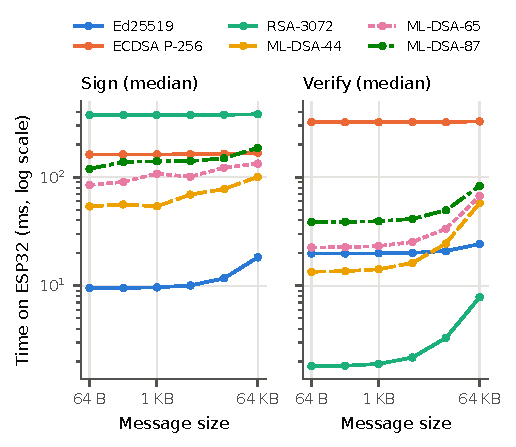
\includegraphics[width=0.62\textwidth]{fig4_size_scaling.pdf}
\caption{Signing and verifying time as the message grows from 64 bytes to 64 KB (median of 100
runs; log scales). The ML-DSA signing lines are uneven because ML-DSA signing time jumps from
run to run (see Step 1).}
\end{figure}

\begin{table}[H]
\centering\small
\begin{tabularx}{\textwidth}{@{}l RRRRRR@{}}
\toprule
Algorithm & 64\,B & 256\,B & 1\,KB & 4\,KB & 16\,KB & 64\,KB \\
\midrule
\multicolumn{7}{@{}l}{\textbf{Sign (median, ms)}} \\
Ed25519     & 9.50   & 9.54   & 9.64   & 10.05  & 11.68  & 18.23 \\
ECDSA P-256 & 162.16 & 162.17 & 162.22 & 162.55 & 163.68 & 168.19 \\
RSA-3072    & 374.33 & 374.26 & 374.28 & 374.69 & 375.62 & 380.39 \\
ML-DSA-44   & 53.79  & 56.04  & 53.85  & 69.08  & 77.79  & 100.57 \\
ML-DSA-65   & 84.76  & 90.36  & 107.72 & 101.12 & 122.21 & 133.38 \\
ML-DSA-87   & 119.33 & 138.33 & 140.06 & 140.70 & 149.71 & 186.38 \\
\midrule
\multicolumn{7}{@{}l}{\textbf{Verify (median, ms)}} \\
Ed25519     & 19.79  & 19.78  & 19.87  & 20.07  & 20.86  & 24.20 \\
ECDSA P-256 & 320.84 & 320.86 & 320.97 & 321.25 & 322.36 & 326.88 \\
RSA-3072    & 1.81   & 1.83   & 1.90   & 2.18   & 3.30   & 7.81 \\
ML-DSA-44   & 13.43  & 13.61  & 14.16  & 16.19  & 24.46  & 57.73 \\
ML-DSA-65   & 22.48  & 22.65  & 23.20  & 25.23  & 33.51  & 66.77 \\
ML-DSA-87   & 38.52  & 38.72  & 39.25  & 41.29  & 49.56  & 82.83 \\
\bottomrule
\end{tabularx}
\caption{Time by message size (median of 100 runs).}
\end{table}

Every algorithm first turns the message into a short ``fingerprint'' (a hash), and only this
step depends on the message size. So the extra time grows in a straight line with the size:

\begin{table}[H]
\centering\small
\begin{tabularx}{0.85\textwidth}{@{}l RR X@{}}
\toprule
Algorithm & Sign: per extra KB & Verify: per extra KB & Why \\
\midrule
ECDSA P-256, RSA-3072 & 0.09\,ms & 0.09\,ms & SHA-256 runs on the ESP32's hardware \\
Ed25519               & 0.14\,ms & 0.07\,ms & SHA-512 on hardware; signing reads the message twice \\
ML-DSA-44, 65, 87     & 0.69\,ms & 0.69\,ms & its hash (SHAKE) runs in software \\
\bottomrule
\end{tabularx}
\caption{Extra time per extra kilobyte of message (straight-line fit; it fits the measurements
almost perfectly, $R^2 = 1.000$). For ML-DSA signing, the per-KB cost of verifying is used: it
is the same hashing work, and ML-DSA's signing times jump too much for a clean fit.}
\end{table}

ML-DSA pays about 7 times more per extra KB than ECDSA and RSA, and the cost is the same for all
three ML-DSA levels. For the small messages a drone sends to authenticate, this is negligible;
for large data (for example a log file) it adds up: verifying 64\,KB with ML-DSA-44 takes
57.7\,ms instead of 13.4\,ms.

% ---------------------------------------------------------------------------
\section{The biggest message the ESP32 can sign}

\begin{table}[H]
\centering\small
\begin{tabularx}{\textwidth}{@{}l R X R R@{}}
\toprule
Algorithm & Biggest message & Why the next size failed & Stack given & Sign time at biggest \\
\midrule
Ed25519     & 110,536\,B & message did not fit in memory & 12,288\,B & 24.2\,ms \\
ECDSA P-256 & 110,536\,B & message did not fit in memory & 11,264\,B & 172.2\,ms \\
RSA-3072    & 110,536\,B & message did not fit in memory & 10,240\,B & 385.3\,ms \\
ML-DSA-44   & 110,536\,B & message did not fit in memory & 23,552\,B & 147.6\,ms \\
ML-DSA-65   & 110,536\,B & message did not fit in memory & 28,672\,B & 443.8\,ms \\
ML-DSA-87   & 110,536\,B & message did not fit in memory & 32,768\,B & 210.4\,ms \\
\bottomrule
\end{tabularx}
\caption{Biggest message that could still be held in memory, signed and verified.}
\end{table}

All six algorithms stopped at exactly the same size. The reason is the ESP32's memory: its
largest single free block was 110,580 bytes, so a bigger message cannot be stored in one piece.
Even the extra memory ML-DSA needs (up to about 24\,KB of stack) fits elsewhere in memory and did
not lower the limit. \textbf{In simple words: for message size, the ESP32's memory is the limit,
not the algorithm.}

% ---------------------------------------------------------------------------
\section{The biggest message that can be signed within a time limit}

A drone often has to finish its work within a fixed time. This table shows the biggest message
each algorithm can sign within 20, 50 or 100\,ms.

\begin{table}[H]
\centering\small
\begin{tabularx}{\textwidth}{@{}l RRRRRR@{}}
\toprule
 & \multicolumn{2}{c}{\textbf{Within 20\,ms}} & \multicolumn{2}{c}{\textbf{Within 50\,ms}} & \multicolumn{2}{c}{\textbf{Within 100\,ms}} \\
\cmidrule(lr){2-3}\cmidrule(lr){4-5}\cmidrule(l){6-7}
Algorithm & usually & 95\% of times & usually & 95\% of times & usually & 95\% of times \\
\midrule
Ed25519     & 79,464 & 79,400 & 110,536 & 110,536 & 110,536 & 110,536 \\
ECDSA P-256 & 0 & 0 & 0 & 0 & 0      & 0 \\
RSA-3072    & 0 & 0 & 0 & 0 & 0      & 0 \\
ML-DSA-44   & 0 & 0 & 0 & 0 & 67,028 & 0 \\
ML-DSA-65   & 0 & 0 & 0 & 0 & 0      & 0 \\
ML-DSA-87   & 0 & 0 & 0 & 0 & 0      & 0 \\
\bottomrule
\end{tabularx}
\caption{Biggest message in bytes (0 = not even a small message). ``Usually'' uses the median
signing time, ``95\% of times'' the 95th percentile. Calculated from the time of a 64-byte
message (Step 1, 1,000 runs) plus the cost per extra KB above, and limited to the 110,536-byte
memory limit.}
\end{table}

Only Ed25519 can always sign a message within 100\,ms (and even within 20\,ms, up to about
79\,KB). ML-DSA-44 usually manages it for messages up to about 67\,KB, but not reliably, because
its signing time jumps from run to run.

% ---------------------------------------------------------------------------
\section{How much data fits next to the signature in one packet}

Drone radios send small packets. A MAVLink packet (the usual drone protocol) carries at most
255 bytes. The signature takes part of that space.

\begin{table}[H]
\centering\small
\begin{tabularx}{\textwidth}{@{}l R RRRR@{}}
\toprule
 & & \multicolumn{4}{c}{\textbf{Room left for data in one packet}} \\
\cmidrule(l){3-6}
Algorithm & Signature & MAVLink 2 (255\,B) & ESP-NOW v1 (250\,B) & ESP-NOW v2 (1,470\,B) & TCP on ESP32 (1,436\,B) \\
\midrule
Ed25519     & 64\,B    & 191\,B & 186\,B & 1,406\,B & 1,372\,B \\
ECDSA P-256 & 72\,B    & 183\,B & 178\,B & 1,398\,B & 1,364\,B \\
RSA-3072    & 384\,B   & none   & none   & 1,086\,B & 1,052\,B \\
ML-DSA-44   & 2,420\,B & none   & none   & none     & none \\
ML-DSA-65   & 3,309\,B & none   & none   & none     & none \\
ML-DSA-87   & 4,627\,B & none   & none   & none     & none \\
\bottomrule
\end{tabularx}
\caption{Data that still fits in ONE packet next to the signature (calculated). ``None'': the
signature alone does not fit, so the message must be split over several packets. Packet sizes:
MAVLink 2 protocol maximum; ESP-NOW and TCP from the ESP32 software used here.}
\end{table}

\begin{figure}[H]
\centering
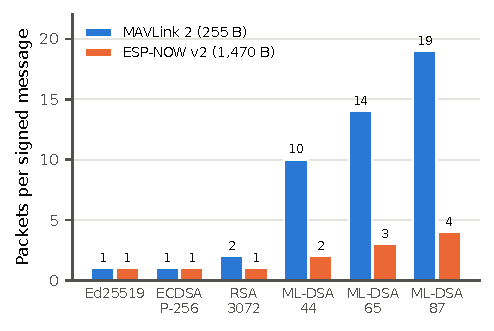
\includegraphics[width=0.62\textwidth]{fig5_packets.pdf}
\caption{Packets needed for one signed authentication message (64 bytes of data plus the
signature). This is the smallest possible number; splitting a message adds a few more header
bytes.}
\end{figure}

With Ed25519 or ECDSA, a whole signed authentication message fits in one drone packet. With
ML-DSA-44 it needs 10 MAVLink packets, and with ML-DSA-87 19. More packets mean more delay, and
if one packet is lost, the whole message fails. \textbf{This is the main practical cost of
post-quantum signatures for drones.}

% ---------------------------------------------------------------------------
\section{Notes and next step}

\textbf{Notes.} At 64 bytes, Step 2 gives slightly different times than Step 1 (ECDSA up to
2.5\%, Ed25519 0.8\%, RSA 0.2\%). Step 2 used 100 runs instead of 1,000 and kept the messages
in a different part of memory. For 64-byte messages, Step 1's numbers are the reference; Step 2
is about how the time grows with size. The packet table is calculated, not yet measured.

\textbf{Next step (Step 3).} The ESP32 will send real signed messages over Wi-Fi to the laptop
(acting as the ground station), with growing amounts of data, for every algorithm. Wireshark
will show how many packets and bytes each message really uses, and exactly where a message stops
fitting in one packet. This measures the packet table above on a real network.

All code, raw measurements and scripts are in the project repository, in
\texttt{Drone\_Auth\_Research/}.

\end{document}
